\subsubsection{Dịch vụ xác thực (auth service - dùng Supabase)}

Hệ thống sử dụng Supabase
để xử lý các nhóm chức năng chính bao gồm:
xác thực và phân quyền,
xác thực 2 yếu tố (MFA),
quản lý dữ liệu người dùng
và quản lý tệp tin
(lưu trữ các file ảnh đại diện do người dùng tải lên tại bucket \texttt{avatars}).
Do mỗi lần người dùng đăng nhập lại,
Supabase/Google sẽ ghi đè lại thông tin gốc từ tài khoản liên kết,
bảng \texttt{profiles} được thiết kế riêng để lưu trữ
và duy trì thông tin của người dùng.
Dưới đây là mô tả chi tiết các chức năng:

\begin{figure}[H]
\centering
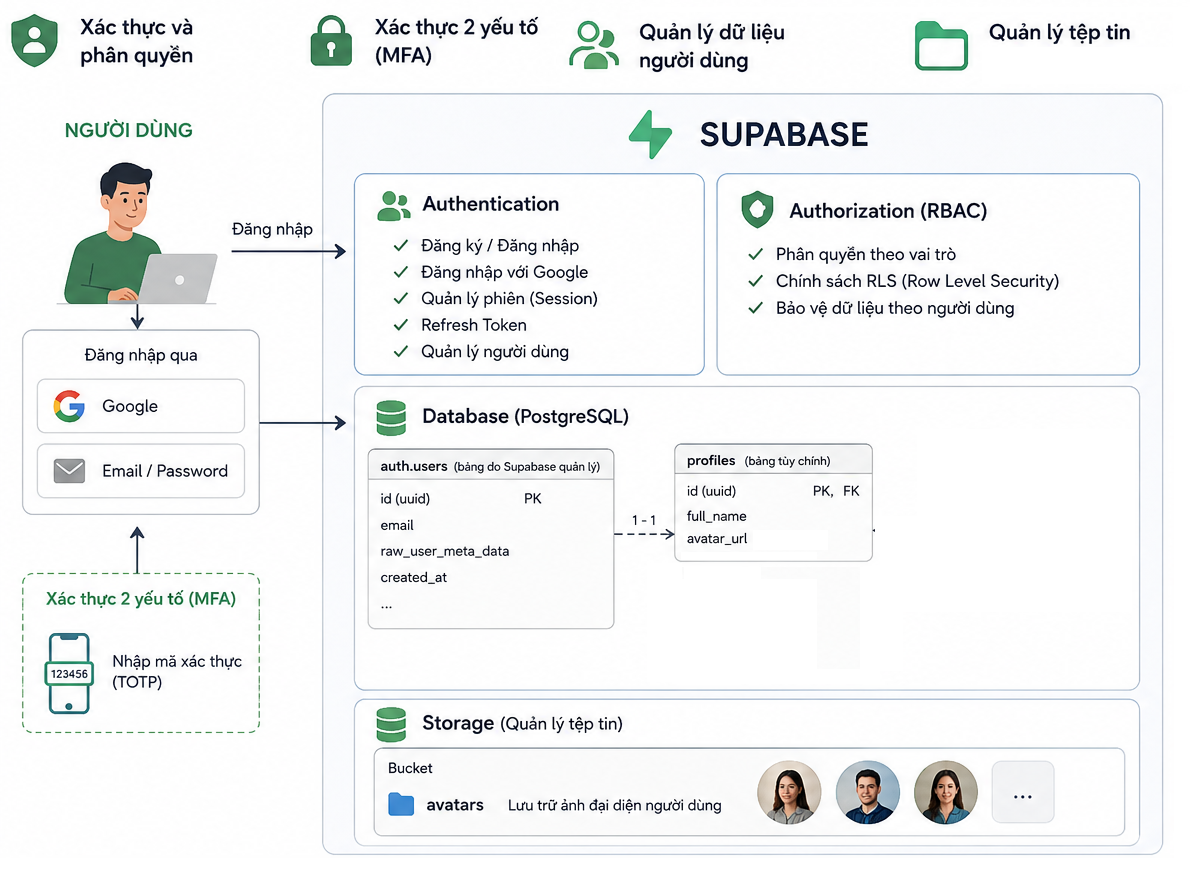
\includegraphics[width=0.99\textwidth]{pictures/supabase-overview.png}
\caption{Tổng quan các chức năng của Supabase}
\end{figure}

\paragraph{Xác thực và quản lý tài khoản}

Hệ thống sử dụng các API Auth của Supabase
để xử lý toàn bộ luồng đăng nhập, đăng ký
và bảo mật tài khoản:

\begin{itemize}

\item \textbf{Đăng nhập bằng Google}:
Tạo URL và chuyển hướng người dùng đến trang ủy quyền của Google.
Endpoint sử dụng: \texttt{/authorize?provider=google}

\item \textbf{Đăng nhập bằng Email và mật khẩu}:
Cho phép người dùng đăng nhập bằng tài khoản email. Trả về thông tin Access Token và Refresh Token nếu thành công.
Endpoint sử dụng: \texttt{/token?grant\_type=password}

\item \textbf{Đăng ký tài khoản mới}:
Tạo tài khoản mới bằng Email và mật khẩu, hỗ trợ gửi email xác nhận tài khoản thông qua đường dẫn chuyển hướng sau khi kích hoạt thành công (\texttt{redirect\_to}).
Endpoint sử dụng: \texttt{/signup}

\item \textbf{Khôi phục mật khẩu}:
Gửi yêu cầu khôi phục mật khẩu tới email của người dùng. Hệ thống sẽ gửi một email chứa liên kết để xác thực và chuyển hướng người dùng về trang đổi mật khẩu.
Endpoint sử dụng: \texttt{/recover}

\item \textbf{Cập nhật mật khẩu mới}:
Cho phép người dùng đổi mật khẩu mới sau khi đã đăng nhập (hoặc sau khi click vào liên kết khôi phục mật khẩu).
Endpoint sử dụng: \texttt{/user}

\item \textbf{Làm mới Access Token}:
Sử dụng \texttt{refresh\_token} để lấy
một \texttt{access\_token} mới
khi token cũ hết hạn.
Endpoint sử dụng: \texttt{/token?grant\_type=refresh\_token}

\item \textbf{Đăng xuất}:
Hủy phiên làm việc hiện tại của người dùng trên hệ thống Supabase.
Endpoint sử dụng: \texttt{/logout}

\end{itemize}

\paragraph{Xác thực 2 yếu tố (MFA)}

Hệ thống hỗ trợ phương thức
xác thực hai yếu tố TOTP (Time-based One-Time Password - như Google Authenticator hay Authy)
bằng các API nâng cao của Supabase:

\begin{itemize}
\item \textbf{Đăng ký thiết bị xác thực MFA mới}:
Khởi tạo quá trình liên kết thiết bị xác thực mới. API trả về mã QR Code (\texttt{qr\_code}), mã bí mật (\texttt{secret}) và chuỗi URI để người dùng quét trên ứng dụng Authenticator.
Endpoint sử dụng: \texttt{/factors}

\item \textbf{Tạo thử thách xác thực}:
Tạo một thử thách xác thực (challenge) dựa trên ID thiết bị MFA (\texttt{factorId}) để chuẩn bị so khớp với mã TOTP người dùng nhập.
Endpoint sử dụng: \texttt{/factors/\{factorId\}/challenge}

\item \textbf{Xác thực mã TOTP}:
Kiểm tra mã TOTP gồm 6 chữ số người dùng nhập có khớp với thử thách hiện tại không. Nếu đúng, Supabase sẽ nâng cấp phiên làm việc của người dùng (tăng cấp bảo mật cho Access Token lên mức độ xác thực \texttt{aal2}).
Endpoint sử dụng: \texttt{/factors/\{factorId\}/verify}

\item \textbf{Lấy danh sách các yếu tố MFA}:
Lấy thông tin tài khoản người dùng để lọc ra danh sách các thiết bị/yếu tố xác thực đã liên kết, phân loại thành: tất cả thiết bị (\texttt{all}) và các thiết bị đã kích hoạt thành công (\texttt{active}).
Endpoint sử dụng: \texttt{/user}

\item \textbf{Hủy liên kết/Xóa thiết bị MFA}:
Xóa một thiết bị xác thực MFA khỏi tài khoản người dùng.
Endpoint sử dụng: \texttt{/factors/\{factorId\}}

\item \textbf{Cập nhật tên hiển thị của thiết bị MFA}:
Đổi tên hiển thị (\texttt{friendly\_name}) của thiết bị xác thực (ví dụ: \enquote{Điện thoại cá nhân}).
Endpoint sử dụng: \texttt{/factors/\{factorId\}}

\end{itemize}

\paragraph{Quản lý Hồ sơ người dùng (Supabase Database - PostgREST API)}

Hệ thống sử dụng cơ chế RESTful API tự động sinh từ PostgreSQL của Supabase (PostgREST) để thực hiện các thao tác CRUD trên bảng CSDL \texttt{profiles}:

\begin{itemize}
\item \textbf{Lấy thông tin hồ sơ}:
Truy vấn thông tin chi tiết hồ sơ người dùng (như tên đầy đủ, ảnh đại diện) từ bảng \texttt{profiles} dựa vào \texttt{userId}.
Endpoint sử dụng: \texttt{/rest/v1/profiles}

\item \textbf{Cập nhật thông tin hồ sơ}:
Cập nhật các trường thông tin hồ sơ như tên hiển thị hoặc đường dẫn ảnh đại diện.
Endpoint sử dụng: \texttt{/rest/v1/profiles}
\end{itemize}

\paragraph{Quản lý Ảnh đại diện (Supabase Storage)}

Hệ thống sử dụng dịch vụ lưu trữ tệp (Storage) của Supabase để quản lý hình ảnh của người dùng:

\begin{itemize}
\item \textbf{Tải lên ảnh đại diện}:
Tải tệp tin ảnh của người dùng lên thư mục \texttt{avatars} trên Supabase Storage. Tên tệp được sinh ngẫu nhiên kết hợp với \texttt{userId} để tránh trùng lặp.
Endpoint tải lên: \texttt{/storage/v1/object/avatars/\{fileName\}}
Đường dẫn công khai nhận về: \texttt{/storage/v1/object/public/avatars/\{fileName\}}
\end{itemize}

Chi tiết về cấu hình Terraform dùng để quản lý hạ tầng Supabase:

\begin{itemize}
\item Sử dụng Terraform Cloud với workspace \texttt{infra-supabase} để lưu trữ và quản lý trạng thái hạ tầng một cách tập trung.

\item Tự động tạo các dự án cho dev và prod dựa trên \texttt{project\_names}.

\item Cấu hình mã vùng (region) là \texttt{ap-southeast-1} tại Singapore để tối ưu tốc độ kết nối cho người dùng tại Việt Nam.

\item Bỏ qua sự thay đổi của mật khẩu nhằm tránh việc Terraform yêu cầu cập nhật hoặc thay đổi mật khẩu CSDL sau mỗi lần chạy cấu hình.

\item Tích hợp đăng nhập qua Google OAuth (Client ID và Client Secret).

\item Thiết lập giới hạn gửi email (rate limit).

\item Cấu hình hệ thống Email (SMTP) đang được cấu hình mặc định là Gmail.

% \item Ghi đè các mẫu email HTML cho "Xác nhận tài khoản" và "Đặt lại mật khẩu" để đồng nhất email tương tự như trong dịch vụ thanh toán.
\item Ghi đè các mẫu email HTML cho \enquote{Xác nhận tài khoản} và \enquote{Đặt lại mật khẩu} để đồng nhất email tương tự như trong dịch vụ thanh toán.
\end{itemize}

\begin{figure}[H]
\centering
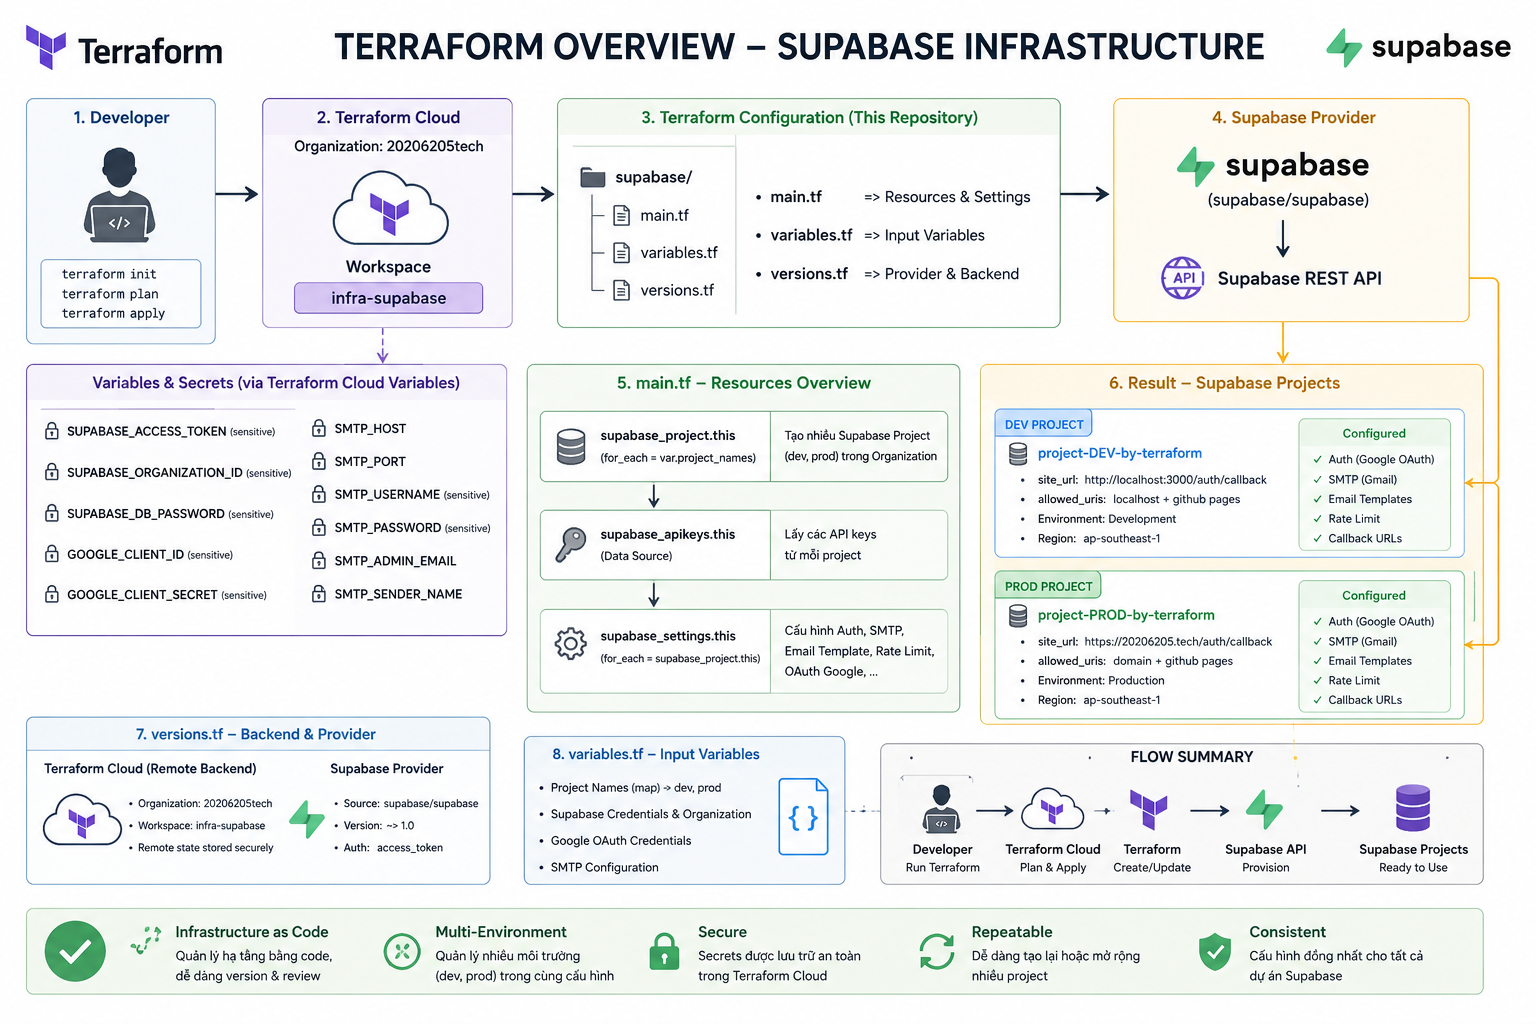
\includegraphics[width=0.95\textwidth]{pictures/auth-terraform-supabase-overview.png}
\caption{Tổng quan cấu hình Terraform quản lý hạ tầng Supabase}
\end{figure}

% \begin{figure}[H]
% \centering
% 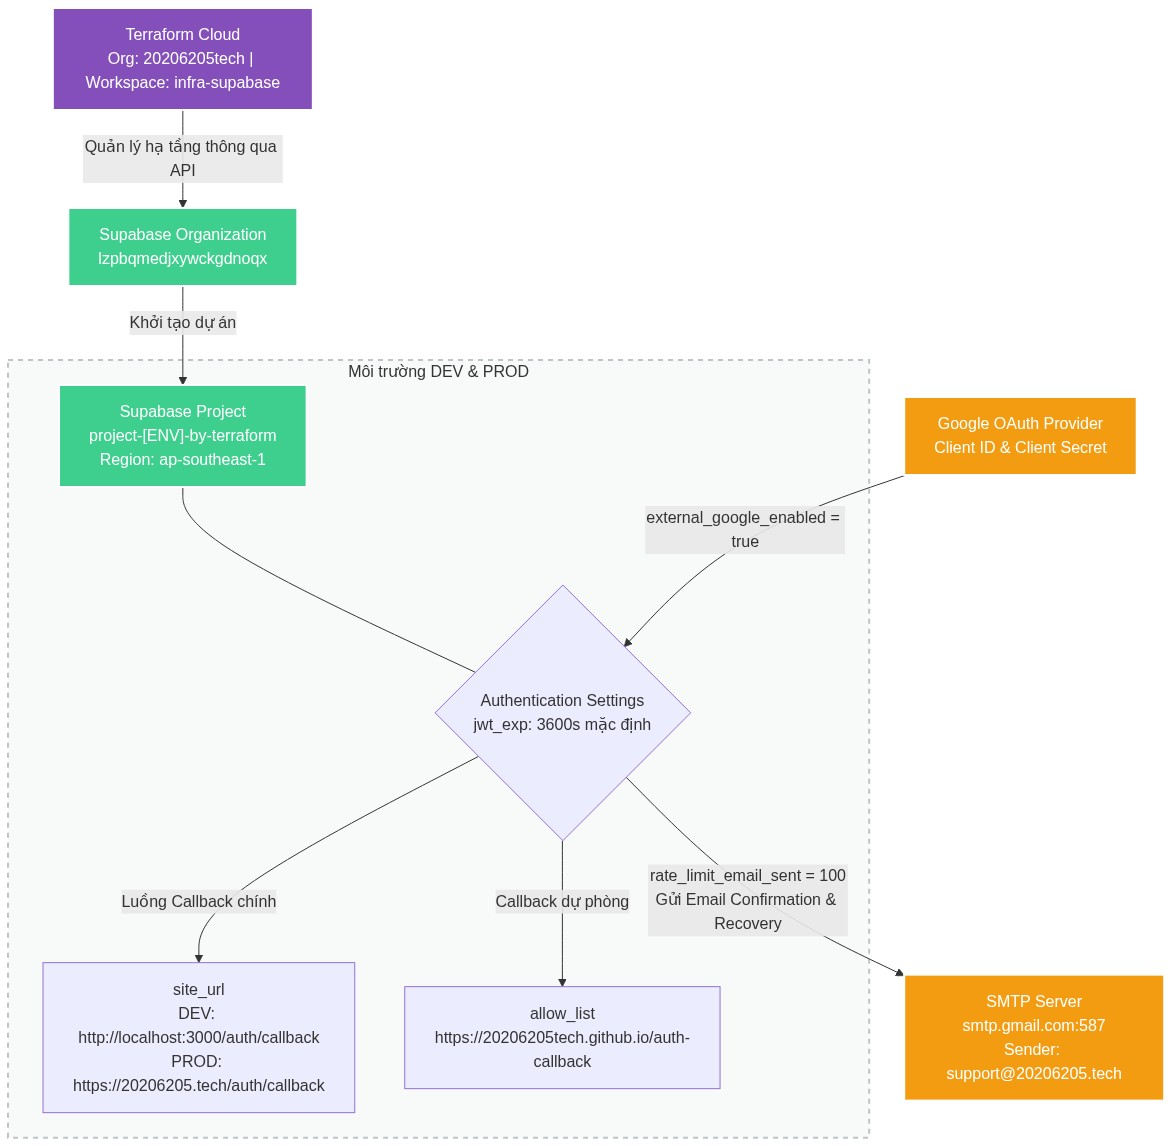
\includegraphics[width=0.65\textwidth]{pictures/auth-terraform-supabase-diagram.png}
% \caption{Sơ đồ cấu hình Terraform cho Supabase}
% \end{figure}

\begin{figure}[H]
\centering
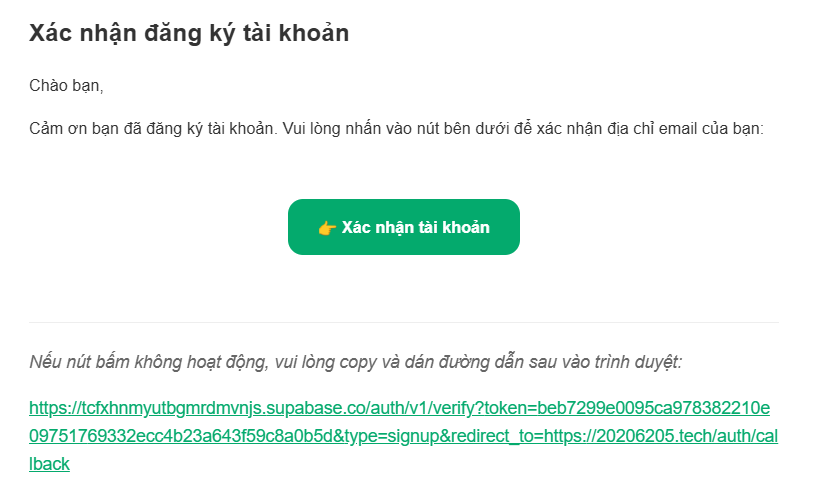
\includegraphics[width=0.8\textwidth]{pictures/auth-mail.png}
\caption{Mẫu email HTML được cấu hình}
\end{figure}

Chi tiết về cấu hình di chuyển CSDL Supabase:

Sử dụng Supabase CLI tạo dự án quản lý di chuyển CSDL bằng lệnh \texttt{npx supabase init}.

Trong thư mục migrations, các file SQL được thiết kế kết hợp với chính sách bảo mật cấp hàng RLS (Row-Level Security):

\begin{itemize}
\item Tạo bảng \texttt{admin\_whitelist} lưu thông tin email của quản trị viên (ADMIN).
\item Tạo bucket \texttt{avatars} lưu thông tin file ảnh đại diện người dùng.
\item Tạo bảng \texttt{profiles} lưu thông tin của người dùng.
\item Tạo bucket \texttt{persona\_avatars} lưu thông tin file ảnh đại diện nhân vật.
\item Tạo bucket \texttt{persona\_audios} lưu thông tin file âm thanh lời chào nhân vật.
\end{itemize}

Kết quả bucket cấu hình trên Supabase:

\begin{figure}[H]
\centering
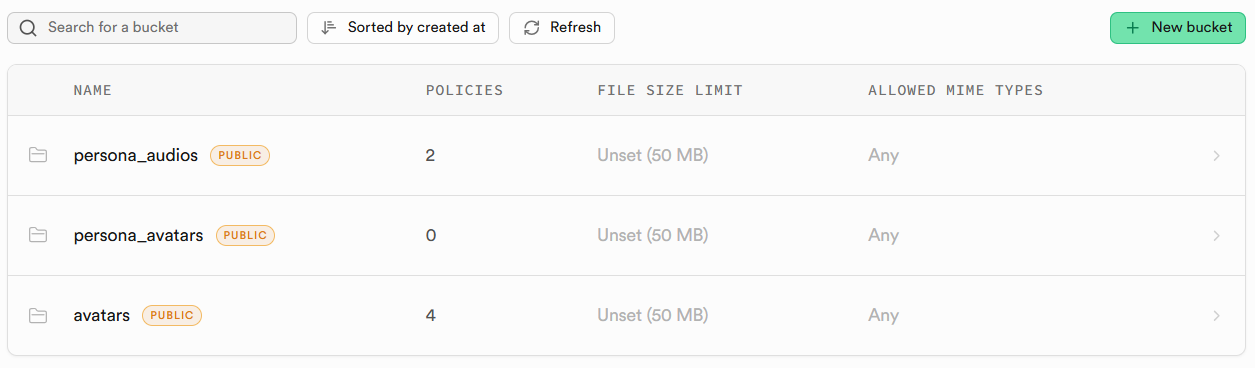
\includegraphics[width=0.95\textwidth]{pictures/auth-supabase-bucket.png}
\caption{Cấu hình các Storage Bucket trên Supabase}
\end{figure}

Kết quả CSDL trên Supabase:

\begin{figure}[H]
\centering
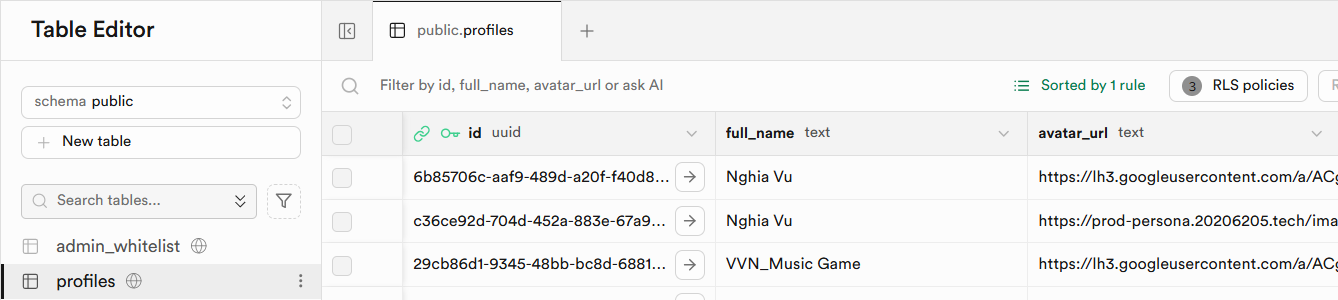
\includegraphics[width=0.95\textwidth]{pictures/auth-supabase-database.png}
\caption{Kết quả bảng CSDL trên Supabase}
\end{figure}

Để tối ưu hóa quá trình phát triển,
các gói thư viện dùng chung (Shared Packages) đã được xây dựng để các dịch vụ khác dễ dàng tái sử dụng và quản lý.
Hiện tại trong dự án, có 2 gói thư viện dùng chung được xây dựng và đăng ký trên npm/PyPI là NestJS (\texttt{20206205tech-nestjs-auth}) và FastAPI trong Python (\texttt{20206205tech-python-auth}). Các thư viện này thực hiện các bước kiểm duyệt bảo mật tự động bao gồm:

\begin{figure}[H]
\centering
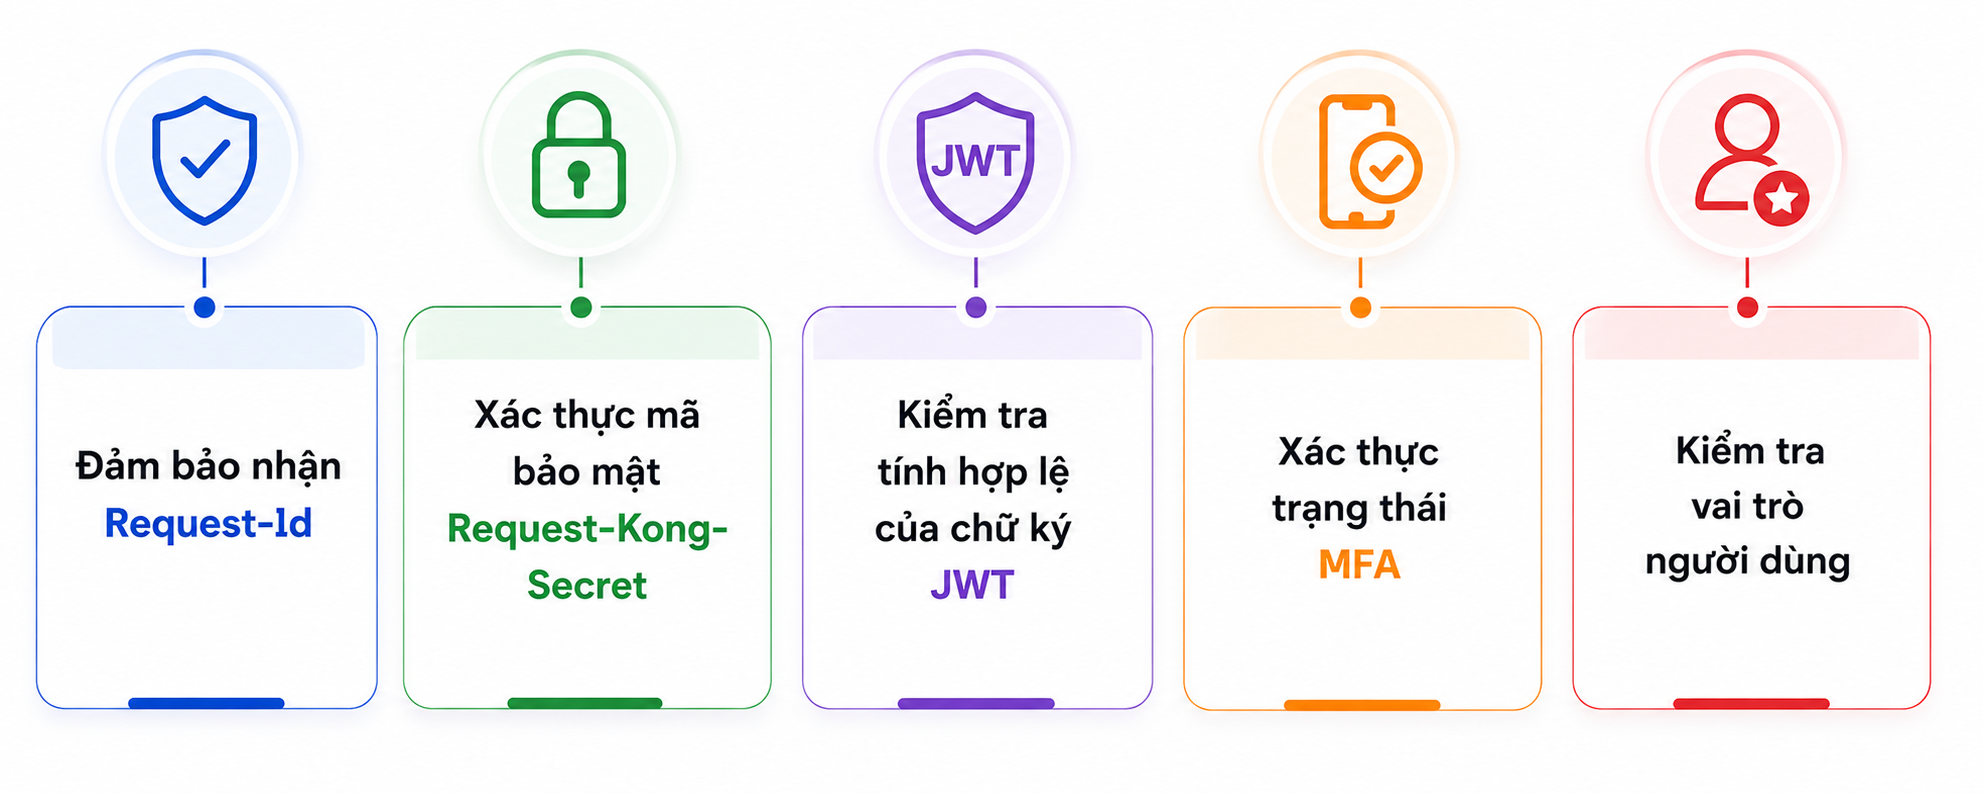
\includegraphics[width=0.9\textwidth]{pictures/auth-common.png}
\caption{Quy trình kiểm tra bảo mật trong gói thư viện dùng chung}
\end{figure}
\begin{itemize}

\item Đảm bảo nhận \texttt{Request-Id} được chuyển tiếp từ Kong API Gateway.
\item Xác thực mã bảo mật \texttt{Request-Kong-Secret} để đảm bảo yêu cầu thực sự đi qua API Gateway.
\item Kiểm tra tính hợp lệ của chữ ký JWT của người dùng thông qua Supabase.
\item Xác thực trạng thái MFA (yêu cầu bắt buộc để nâng cao bảo mật dữ liệu).
\item Kiểm tra vai trò người dùng (ví dụ: yêu cầu vai trò quản trị viên ADMIN đối với các API quản lý).
\end{itemize}

Kết quả sơ đồ tệp và thư mục trong gói chung NestJS Auth được tạo tự động từ depcruise:

\begin{figure}[H]
\centering
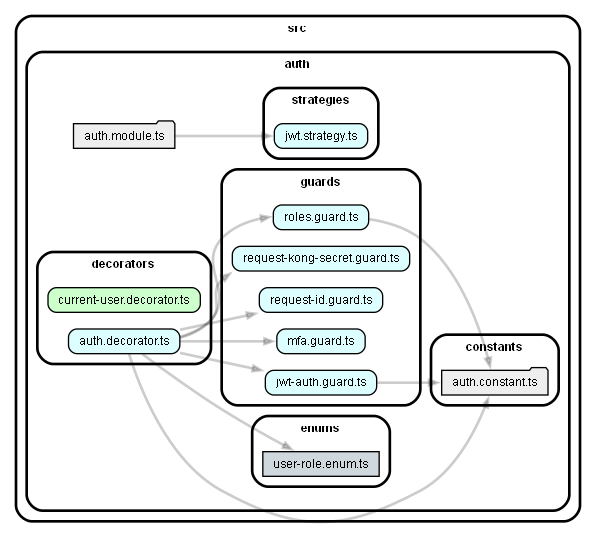
\includegraphics[width=0.6\textwidth]{pictures/20206205tech-nestjs-auth-file-architecture.png}
\caption{Sơ đồ tệp và thư mục trong gói chung NestJS}
\end{figure}

\paragraph{Cấu hình trong Kong API Gateway}

Tạo Service trong Kong trỏ về URL của dự án Supabase (\texttt{https://[PROJECT\_REF].supabase.co}).
Thiết lập Route: Tạo một Route liên kết với Service vừa tạo.
Tham số \texttt{strip\_path=true} đảm bảo Kong sẽ xóa tiền tố khỏi URI trước khi chuyển tiếp yêu cầu đến Supabase.
Dùng plugin \texttt{request-transformer} để tự động thêm \texttt{apikey} vào header trước khi gửi đến Supabase.
